% Bagian Lampiran
\section*{Lampiran} % Jika ada lampiran

\begin{figure}[h]
  \centering
  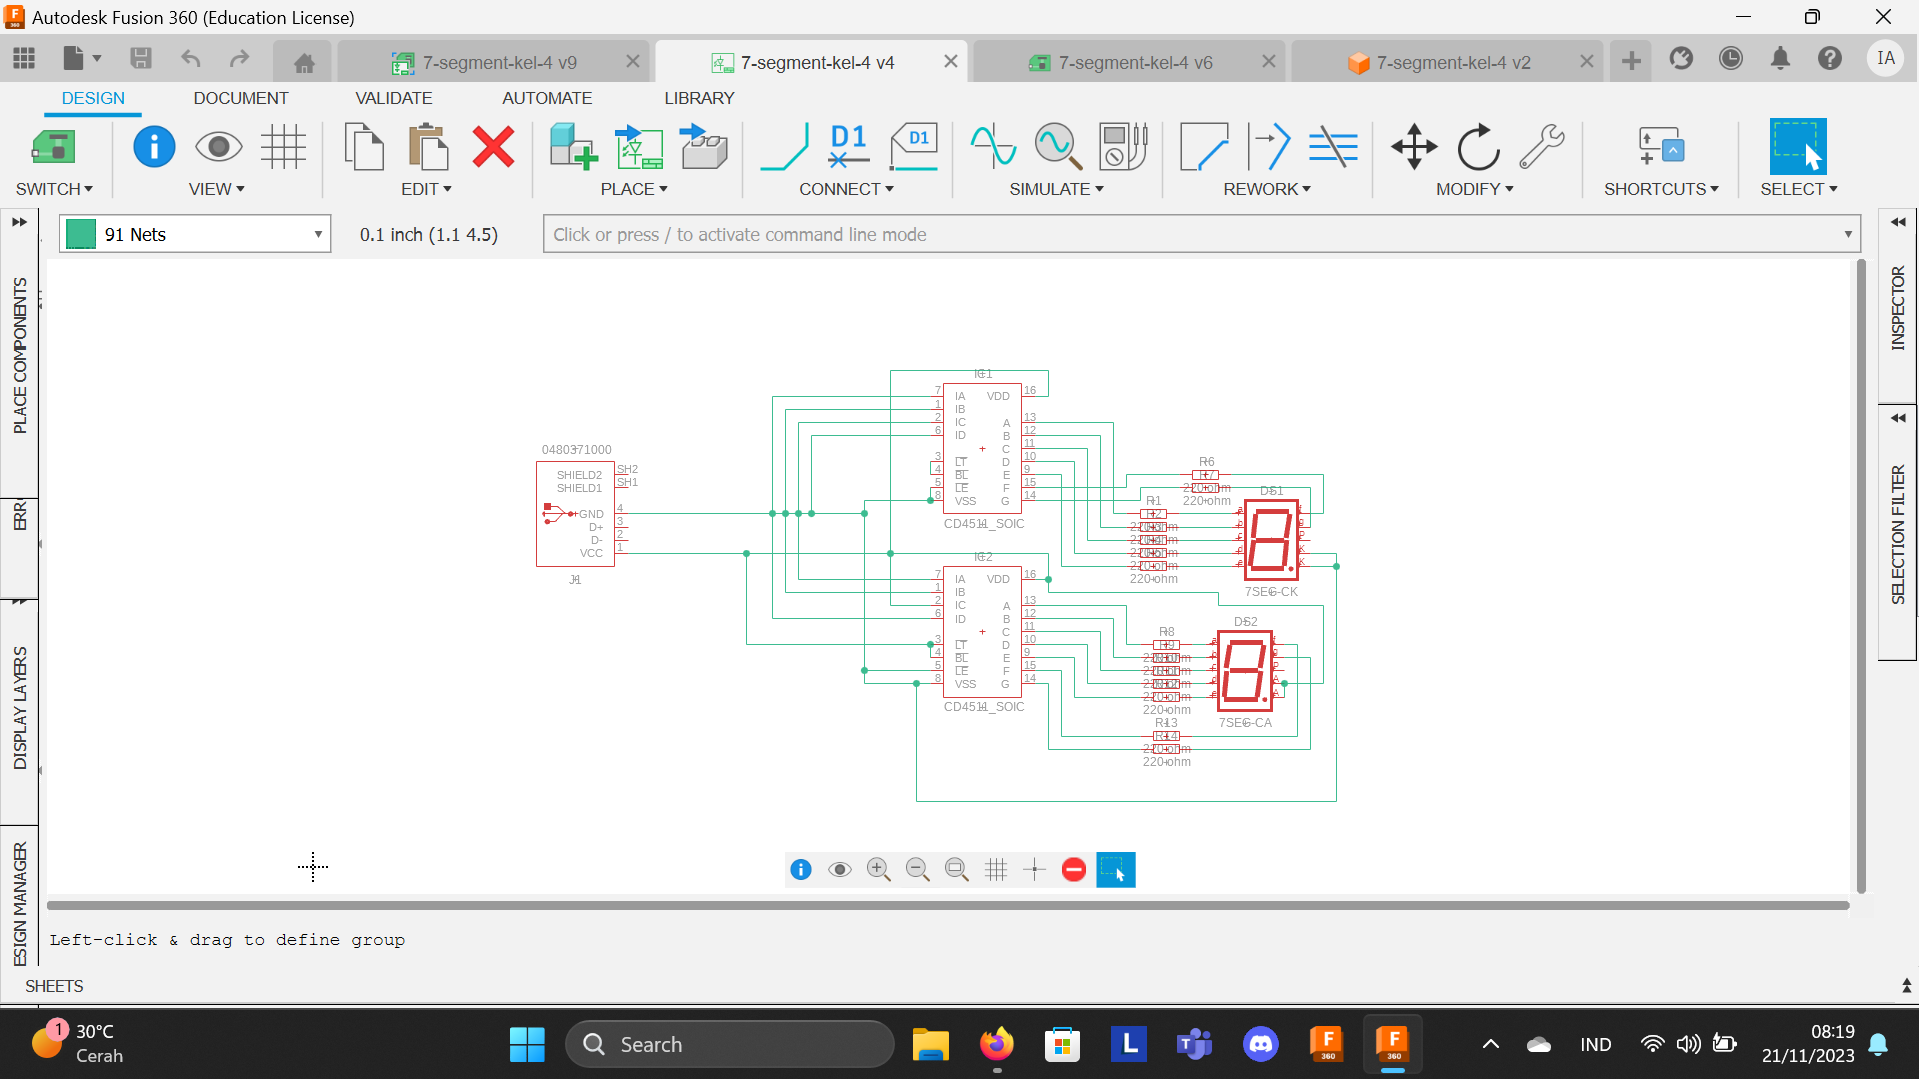
\includegraphics[width=0.45\linewidth]{img/raw-circuit.png}
  \caption{Rangkaian digital yang digunakan untuk menampilkan nomor kelompok} 
  \label{fig:raw-circuit}
\end{figure}

\begin{figure}[h]
  \centering
  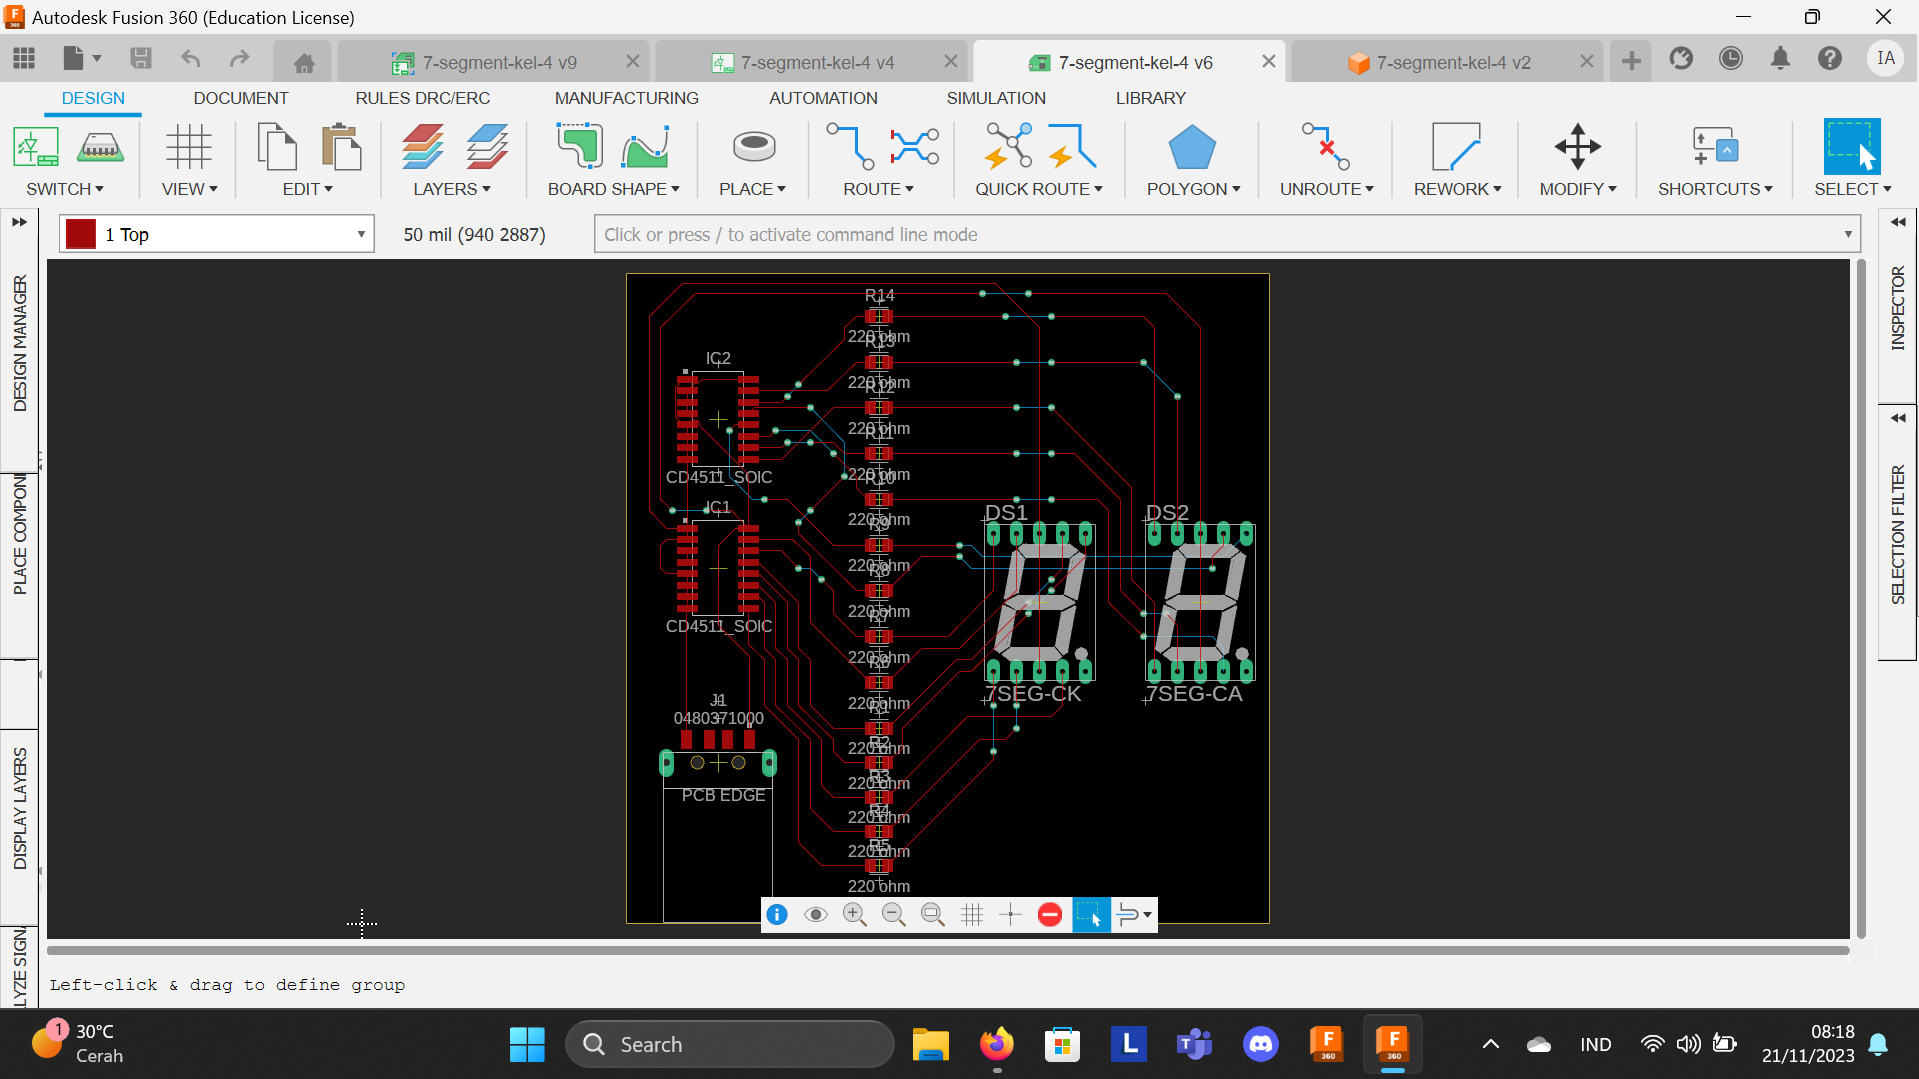
\includegraphics[width=0.5\linewidth]{img/wired-schematic.png}
  \caption{Schematic yang digunakan untuk menampilkan nomor kelompok} 
  \label{fig:wired-schematic}
\end{figure}

\begin{figure}[h]
  \centering
  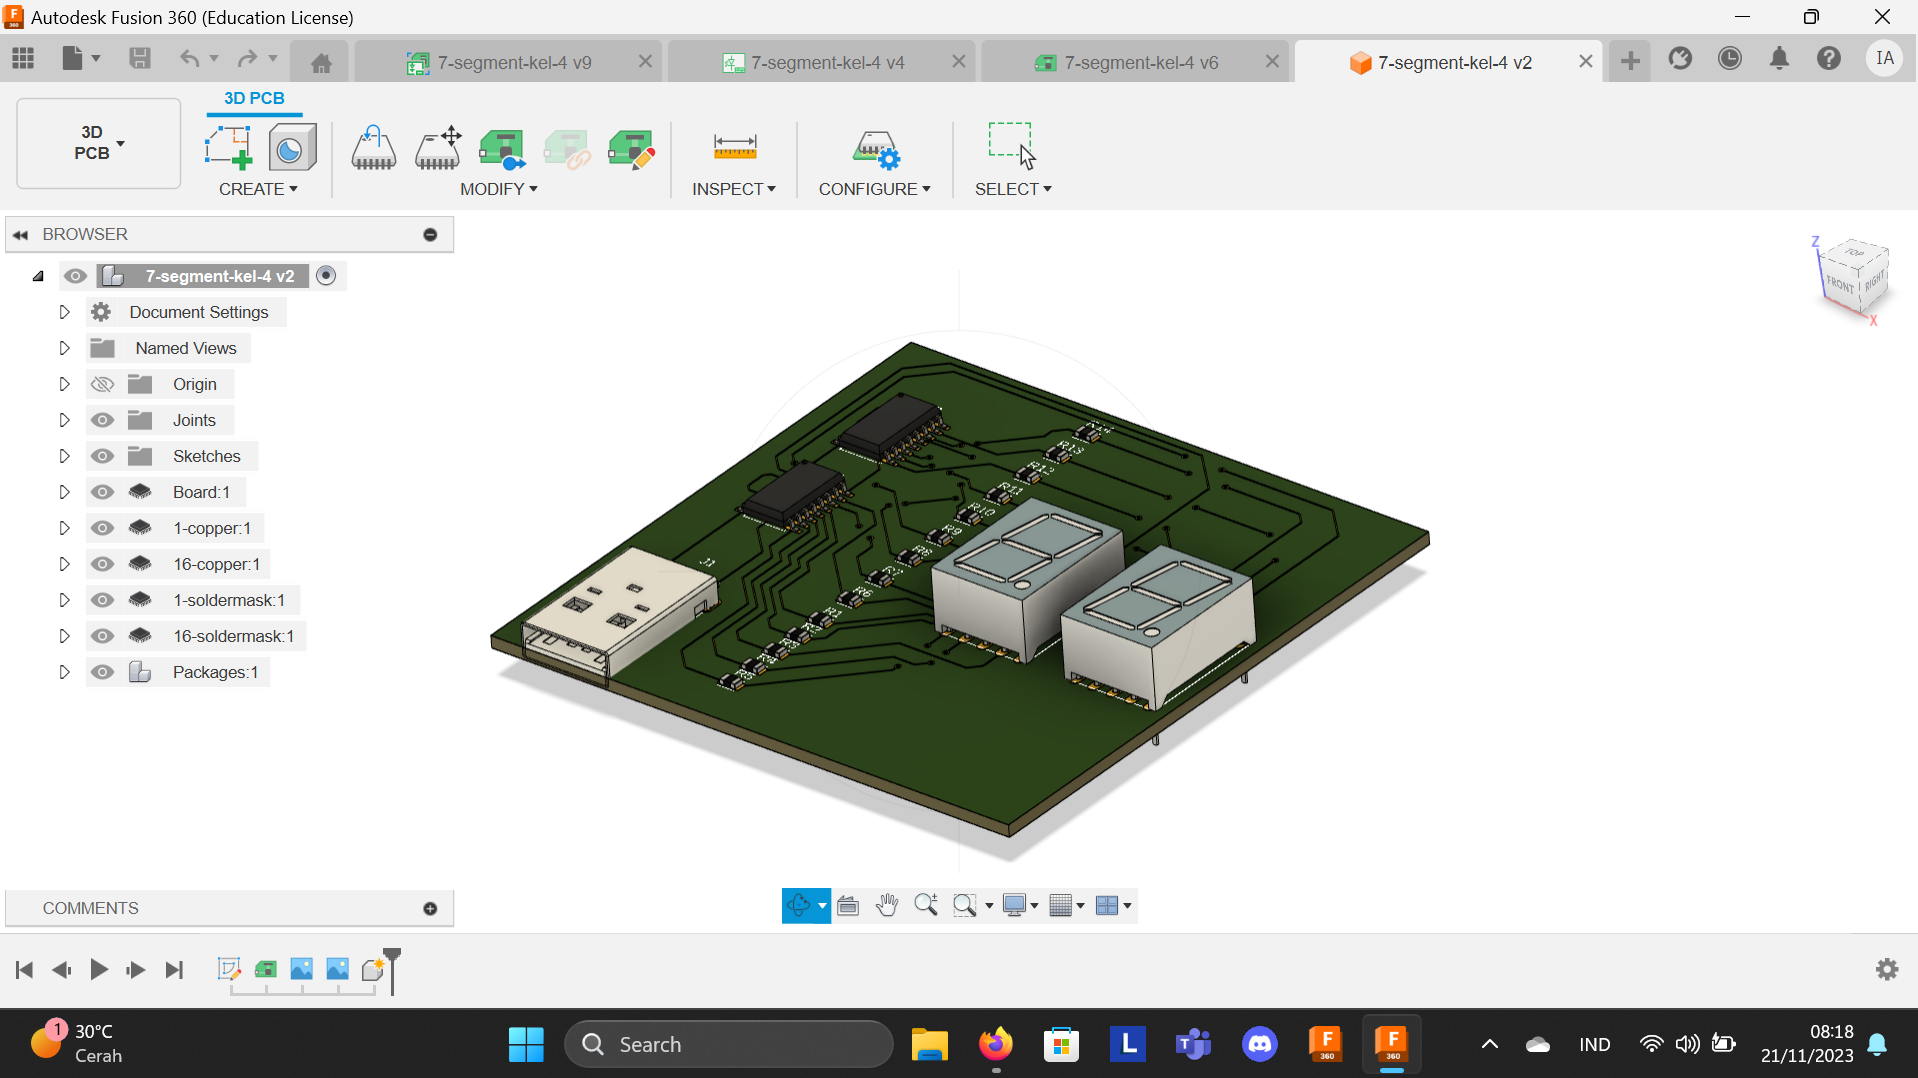
\includegraphics[width=0.5\linewidth]{img/3d-7segment.png}
  \caption{3D view dari schematic yang digunakan untuk menampilkan nomor kelompok} 
  \label{fig:3d-schematic}
\end{figure}

\begin{figure}[h]
  \centering
  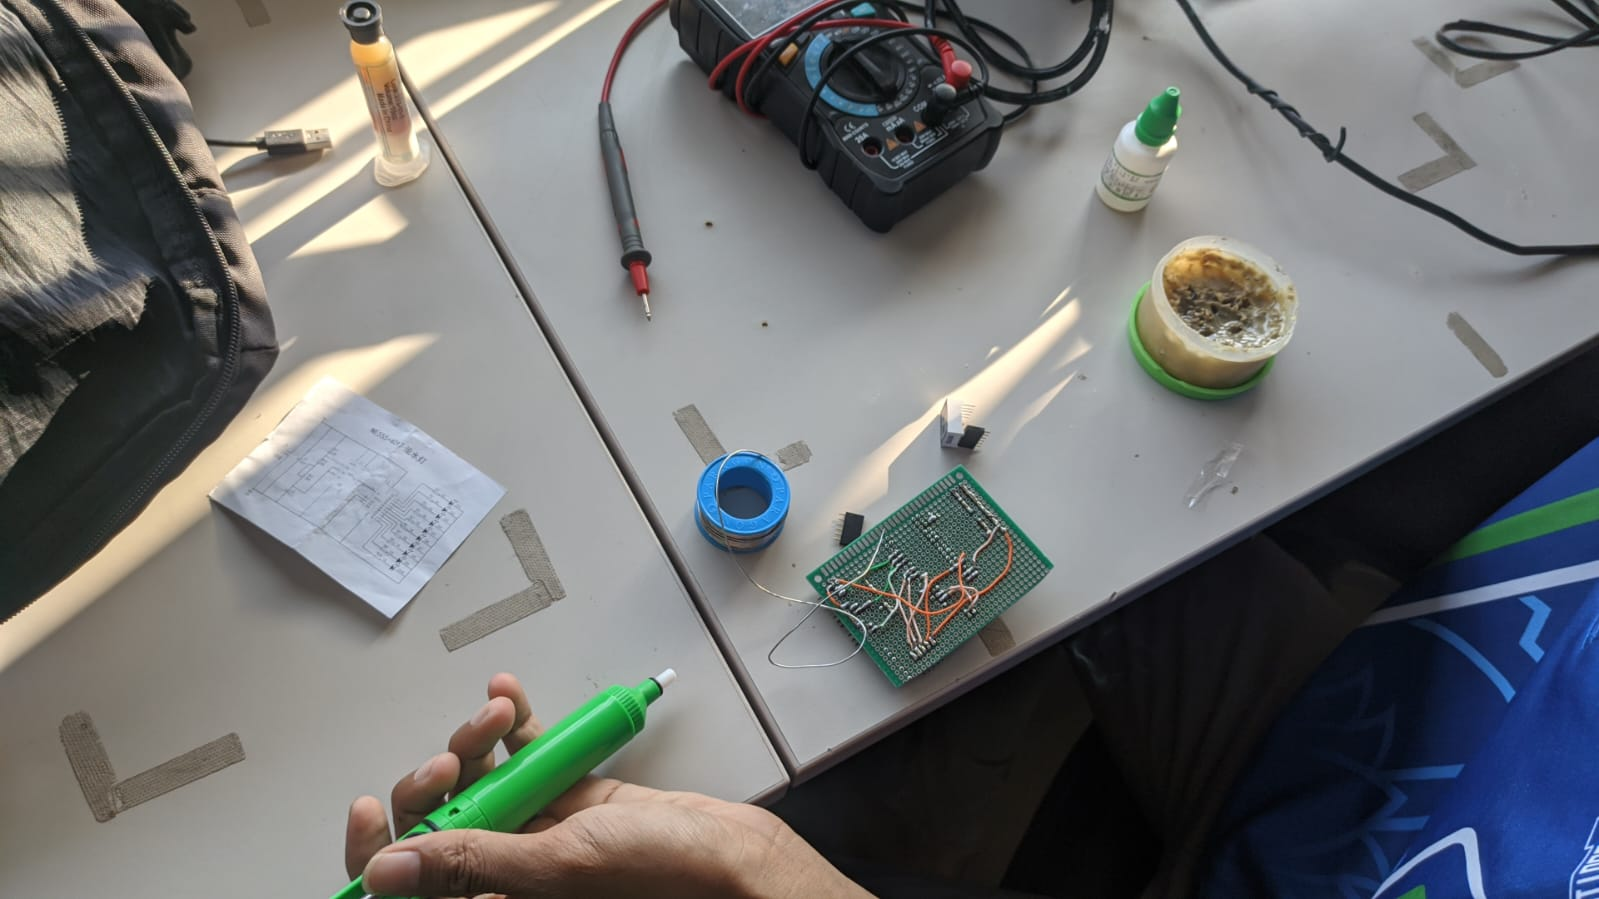
\includegraphics[width=0.8\linewidth]{img/soldering-ce.jpeg}
  \caption{Proses soldering PCB biasa} 
  \label{fig:soldering-ce}
\end{figure}

\begin{figure}[h]
  \centering
  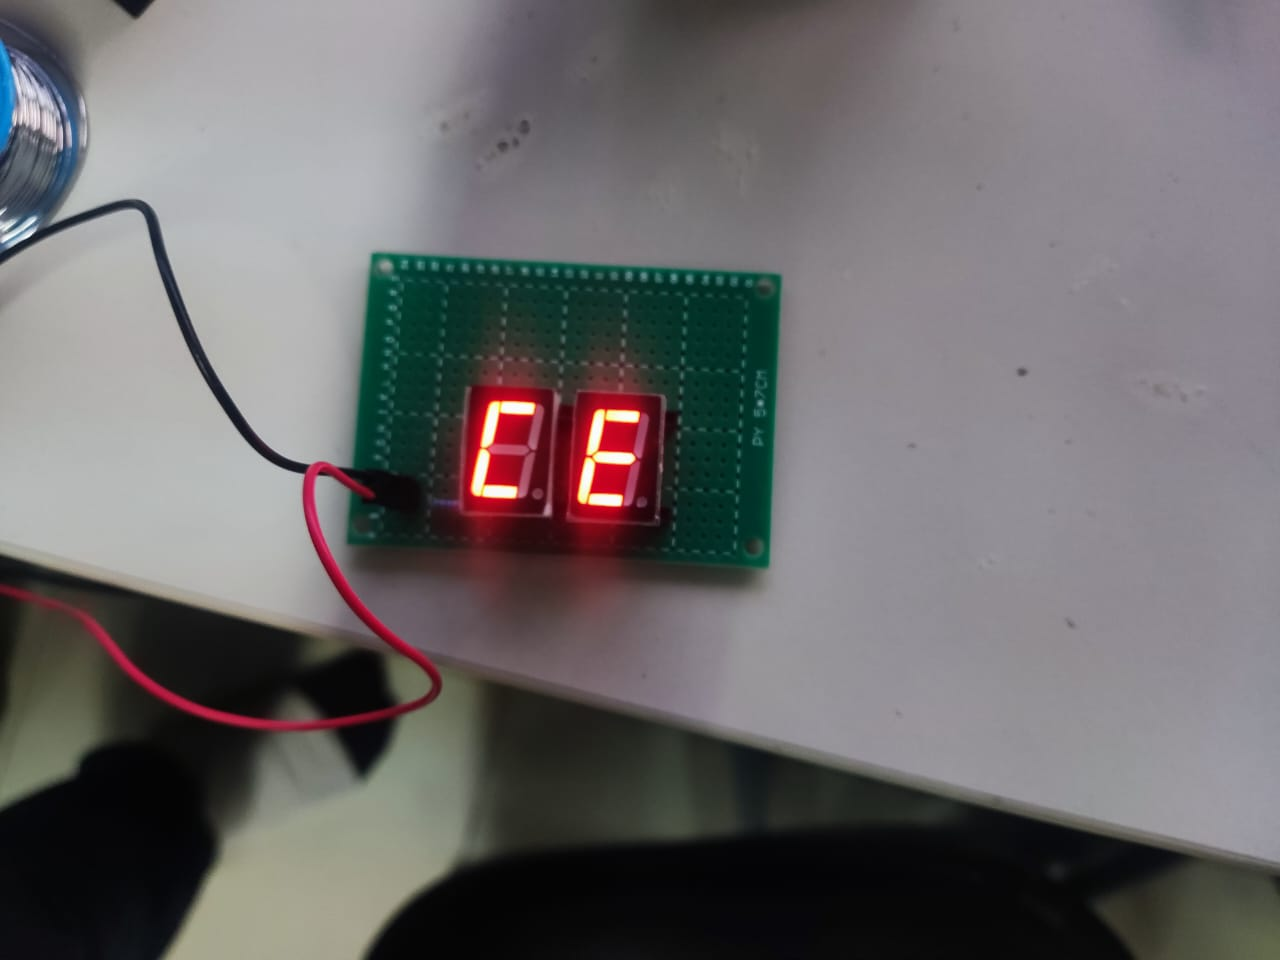
\includegraphics[width=0.8\linewidth]{img/ce-result.jpeg}
  \caption{Hasil soldering 7-segment dengan output CE} 
  \label{fig:ce-result}
\end{figure}

\begin{figure}[h]
  \centering
  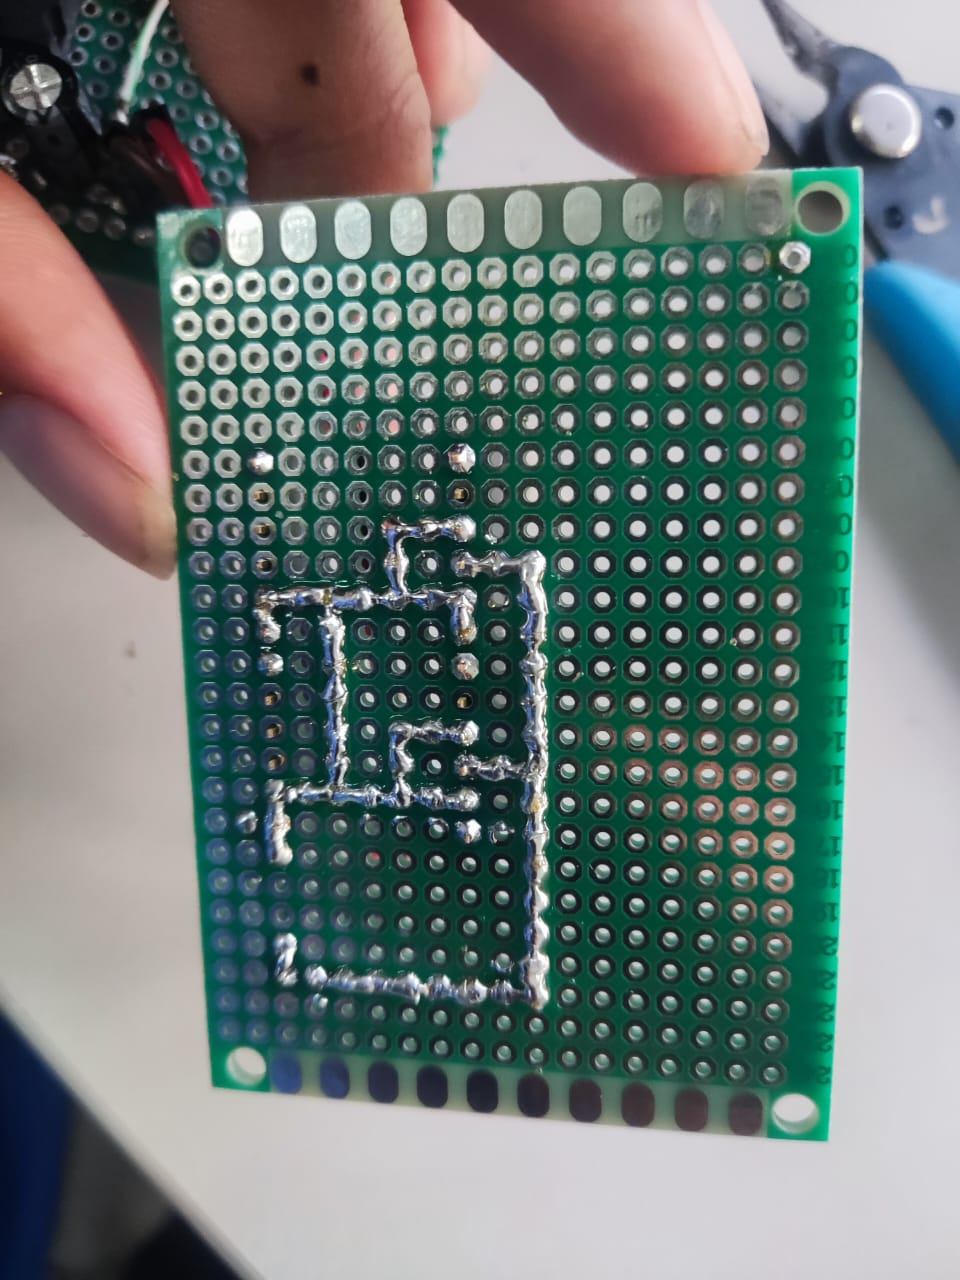
\includegraphics[width=0.6\linewidth]{img/cd-result-back.jpeg}
  \caption{Jalur timah dari hasil solder 7-segment} 
  \label{fig:ce-result-back}
\end{figure}

\begin{figure}[h]
  \centering
  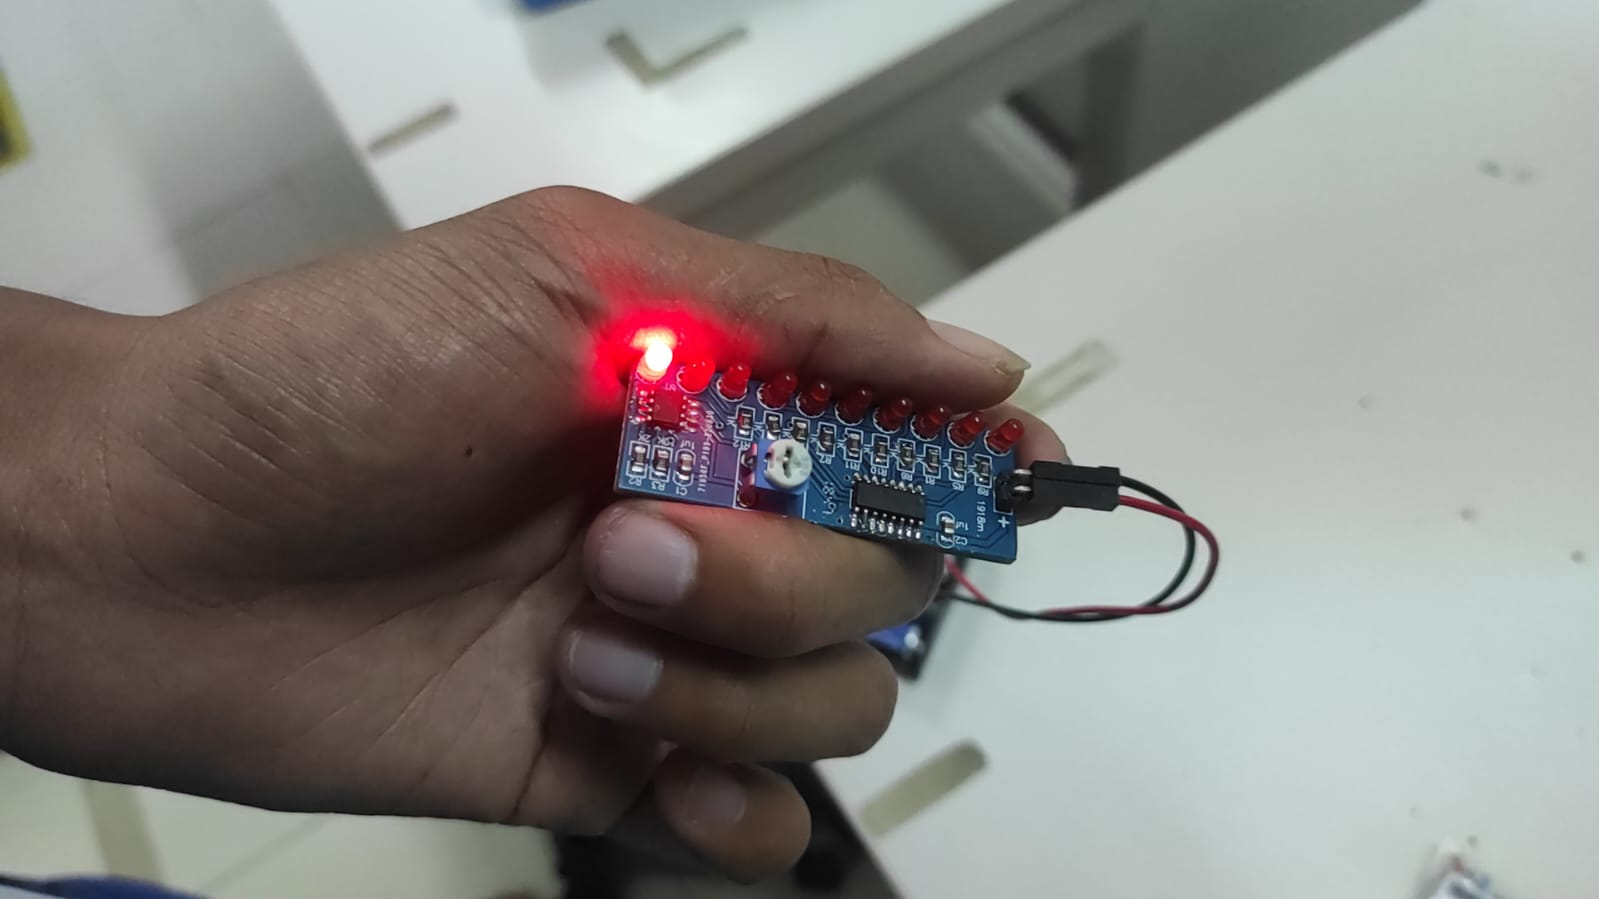
\includegraphics[width=0.6\linewidth]{img/smd-front.jpeg}
  \caption{Hasil solder komponen SMD dan output-nya} 
  \label{fig:smd-front}
\end{figure}

\begin{figure}[h]
  \centering
  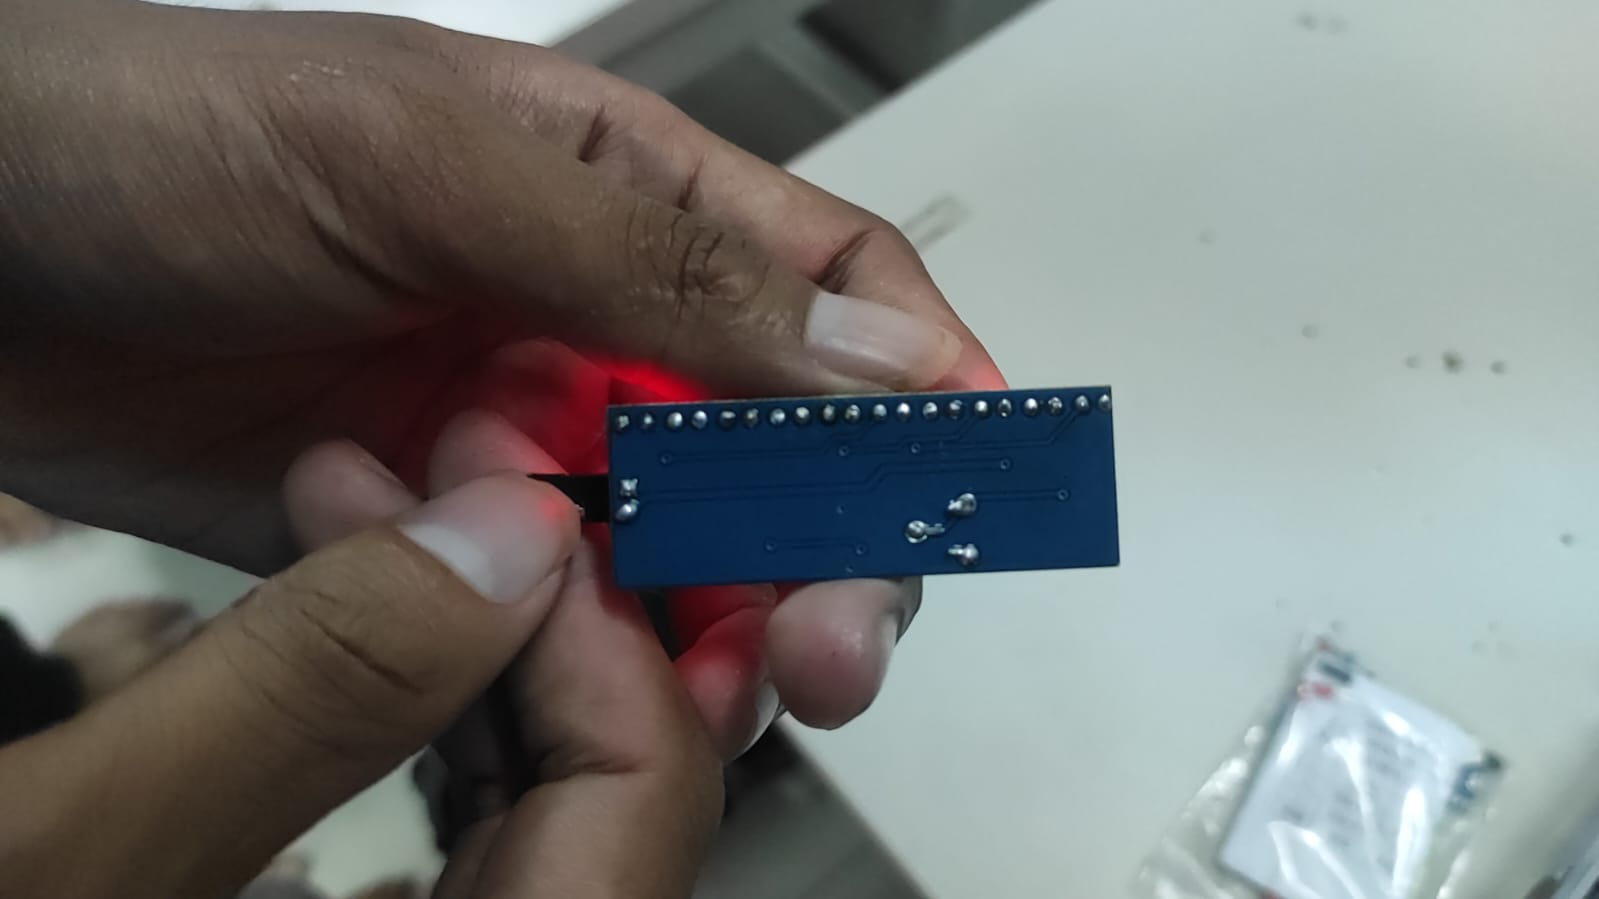
\includegraphics[width=0.8\linewidth]{img/smd-back.jpeg}
  \caption{Tampak belakang SMD} 
  \label{fig:smd-back}
\end{figure}

% \begin{figure}[H]
%   \centering
%   
\includegraphics[width=0.2\linewidth]{img/contohgambar.png}
%   \caption{Ini Caption} 
%   \label{fig:inirujukan}
% \end{figure}
% \vspace{0pt}
% \begin{figure}[H]
%   \centering
%   % Kalau mau menambah gambar lagi tinggal nambahin begin{subfigure} -> end{subfigure}
%   \begin{subfigure}[b]{0.4\linewidth}
%     \centering
%     
\includegraphics[width=\linewidth]{img/contohgambar.png}
%     \caption{Ini Caption sub 1\label{fig:inisub1}}
%   \end{subfigure}
%   \hspace{1cm}
%   \begin{subfigure}[b]{0.4\linewidth}
%     \centering
%     
\includegraphics[width=\linewidth]{img/contohgambar.png}
%     \caption{Ini Caption sub 2\label{fig:inisub2}}
%   \end{subfigure}
%   \caption{Caption kedua gambar\label{fig:keduagambar}}
% \end{figure}